% !Mode:: "TeX:UTF-8"
% !TeX program = xelatex
\documentclass[bachelor,ktreport,openany,oneside,AutoFakeBold=true]{buaathesis}

\usepackage{float}
\usepackage{tikz}
\usepackage{upquote}

\usetikzlibrary{arrows.meta,positioning,shapes.geometric}

\setmonofont{Consolas}
\graphicspath{{figures/}{figure/}}
\setlength{\headheight}{16pt}
\hypersetup{
  hidelinks,
  pdftitle={实验一：时域采样与频域采样},
  pdfauthor={傅粱训},
  pdfsubject={数字信号处理实验报告}
}

\newcommand{\Hz}{\mathrm{Hz}}
\newcommand{\dd}{\mathrm{d}}

\begin{document}

\degree{数字信号处理实验}{Course}{数字信号处理实验}{数字信号处理实验}
\ktclass{数字信号处理实验报告}
\school{未来空天技术}{School of Future Aerospace Technology}
\major{工科试验班（未来空天领军计划）}{Engineering Experimental Class}
\class{242311班}
\thesistitle{实验一：时域采样与频域采样}{}{Experiment 1: Time-domain Sampling and Frequency-domain Sampling}{}
\studentID{24373088}
\thesisauthor{傅粱训}{Fu Liangxun}
\teacher{白桐老师}{Bai Tong}
\thesisdate{2026}{6}

\ckeyword{时域采样；频域采样；FFT；频谱混叠；周期延拓}
\ekeyword{time-domain sampling; frequency-domain sampling; FFT; aliasing; periodic extension}

\pagestyle{mainmatter}
\maketitle

\pagestyle{frontmatter}
\begin{cabstract}
本实验围绕时域采样和频域采样两个基本理论展开。通过对指数衰减正弦模拟信号进行不同采样频率下的离散化和 FFT 分析，观察采样前后频谱的变化，理解采样频率不足时产生频谱混叠的原因。实验分别取 \(F_s=1000\,\Hz\)、\(300\,\Hz\) 和 \(200\,\Hz\)，在 \(T_p=50\,\mathrm{ms}\) 的观测时间内生成采样序列，并统一采用 64 点 FFT 绘制幅频特性。

实验还对长度为 \(M=27\) 的有限长三角序列进行频域采样验证。通过对其频谱分别进行 32 点和 16 点等间隔采样，并作 IFFT，比较原序列、\(x_{32}(n)\) 和 \(x_{16}(n)\) 的波形。结果表明，当频域采样点数 \(N\ge M\) 时，时域不发生混叠；当 \(N<M\) 时，IFFT 结果为原序列按 \(N\) 周期折叠后的主值区叠加序列。实验验证了“时域采样导致频域周期延拓，频域采样导致时域周期延拓”的对偶关系。
\end{cabstract}

\begin{eabstract}
This experiment studies two basic sampling theorems in digital signal processing. An exponentially decaying sinusoidal analog signal is sampled at different sampling rates, and its spectra are analyzed with a 64-point FFT. The results show that a higher sampling rate enlarges the spacing between periodic spectral replicas, while an insufficient sampling rate causes aliasing distortion.

The experiment also verifies the frequency-domain sampling theorem with a finite-length triangular sequence of length \(M=27\). The spectrum is sampled with 32 and 16 equally spaced frequency samples, followed by IFFT reconstruction. The 32-point result preserves the original sequence with zero padding, whereas the 16-point result becomes the periodic alias sum of the original sequence. The results confirm the duality between time-domain sampling and frequency-domain sampling.
\end{eabstract}

\tableofcontents
\cleardoublepage
\phantomsection
\addcontentsline{toc}{chapter}{图目录}
\listoffigures
\cleardoublepage
\phantomsection
\addcontentsline{toc}{chapter}{表目录}
\listoftables

\mainmatter
\pagestyle{mainmatter}

\chapter{实验目的}

本实验围绕时域采样和频域采样两个基本理论展开。通过对模拟信号进行不同采样频率下的离散化和 FFT 分析，观察采样前后频谱的变化，理解采样频率不足时产生频谱混叠的原因。通过对有限长序列频谱进行 32 点和 16 点等间隔采样，并分别作 IFFT，验证频域采样会导致时域序列按采样点数进行周期延拓；当频域采样点数小于原序列长度时，时域会发生混叠失真。

\chapter{实验原理}

\section{时域采样定理}

设模拟信号为 \(x_a(t)\)，以采样周期 \(T\) 进行理想采样，采样角频率为
\begin{equation}
\Omega_s=\frac{2\pi}{T}.
\end{equation}
理想采样信号可写为
\begin{equation}
\hat{x}_a(t)=\sum_{n=-\infty}^{\infty}x_a(nT)\delta(t-nT).
\end{equation}
其频谱为原模拟信号频谱的周期延拓：
\begin{equation}
\hat{X}_a(j\Omega)=\frac{1}{T}\sum_{m=-\infty}^{\infty}
X_a\left[j(\Omega-m\Omega_s)\right].
\end{equation}
因此，时域采样会使频域频谱以 \(\Omega_s\) 为周期重复。当采样角频率满足
\begin{equation}
\Omega_s \ge 2\Omega_m
\end{equation}
时，采样后频谱不发生混叠，其中 \(\Omega_m\) 为信号最高角频率。若采样频率不足，则周期延拓的频谱相互重叠，产生频谱混叠失真。

在计算机实验中，模拟信号经采样得到离散序列
\begin{equation}
x(n)=x_a(nT).
\end{equation}
序列的 DTFT 与理想采样信号频谱之间满足变量替换关系
\begin{equation}
\omega=\Omega T,
\end{equation}
因此可以用 FFT 近似观察采样序列的幅频特性。

\section{频域采样定理}

对离散序列 \(x(n)\) 的频谱 \(X(e^{j\omega})\) 在 \([0,2\pi]\) 上等间隔采样 \(N\) 点：
\begin{equation}
X_N(k)=X\left(e^{j\frac{2\pi k}{N}}\right),\quad k=0,1,\cdots,N-1.
\end{equation}
对 \(X_N(k)\) 作 \(N\) 点 IDFT，得到
\begin{equation}
x_N(n)=\mathrm{IDFT}\{X_N(k)\}
=\sum_{r=-\infty}^{\infty}x(n+rN),\quad n=0,1,\cdots,N-1.
\end{equation}
由此可知，频域采样会导致时域序列按 \(N\) 为周期进行延拓并在主值区相加。若原序列长度为 \(M\)，当 \(N\ge M\) 时不会发生时域混叠；当 \(N<M\) 时，不同周期的样值会叠加到同一主值区位置，产生时域混叠。

时域采样与频域采样具有对偶性：时域采样导致频域周期延拓，频域采样导致时域周期延拓。

\chapter{实验内容与结果分析}

\section{主程序框图}

实验主程序流程如图 \ref{fig:flowchart1} 所示。程序首先设置采样参数并生成三组采样序列，然后用 64 点 FFT 观察不同采样频率下的幅频特性；接着构造有限长三角序列，分别进行 32 点和 16 点频域采样，并通过 IFFT 验证频域采样引起的时域周期延拓。

\begin{figure}[H]
\centering
\begin{tikzpicture}[
  node distance=8mm,
  process/.style={rectangle, draw, rounded corners=2pt, align=center, minimum width=10.2cm, minimum height=9mm},
  startstop/.style={ellipse, draw, align=center, minimum width=3.0cm, minimum height=8mm},
  arrow/.style={-{Stealth[length=2.2mm]}, thick}
]
\node[startstop] (start) {开始};
\node[process, below=of start] (param) {设置 \(A,\alpha,\Omega_0,T_p\)，选取 \(F_s=1000,300,200\,\Hz\)};
\node[process, below=of param] (sample) {按 \(x(n)=x_a(nT)\) 生成三组时域采样序列};
\node[process, below=of sample] (fft) {对三组序列补零并作 64 点 FFT，绘制时域波形和幅频特性};
\node[process, below=of fft] (freq) {构造有限长序列 \(x(n)\)，计算 32 点和 16 点频域采样};
\node[process, below=of freq] (ifft) {分别作 IFFT，比较 \(x(n)\)、\(x_{32}(n)\)、\(x_{16}(n)\)};
\node[process, below=of ifft] (analysis) {分析频谱混叠和时域周期混叠现象};
\node[startstop, below=of analysis] (end) {结束};

\draw[arrow] (start) -- (param);
\draw[arrow] (param) -- (sample);
\draw[arrow] (sample) -- (fft);
\draw[arrow] (fft) -- (freq);
\draw[arrow] (freq) -- (ifft);
\draw[arrow] (ifft) -- (analysis);
\draw[arrow] (analysis) -- (end);
\end{tikzpicture}
\caption{实验一主程序框图}
\label{fig:flowchart1}
\end{figure}

\section{时域采样理论验证}

实验给定模拟信号为
\begin{equation}
x_a(t)=Ae^{-\alpha t}\sin(\Omega_0t)u(t),
\end{equation}
其中
\begin{equation}
A=444.128,\quad \alpha=50\sqrt{2}\pi,\quad
\Omega_0=50\sqrt{2}\pi\,\mathrm{rad/s}.
\end{equation}
取观测时间 \(T_p=50\,\mathrm{ms}\)，分别采用三种采样频率
\[
F_s=1000\,\Hz,\quad 300\,\Hz,\quad 200\,\Hz.
\]
采样序列长度按
\begin{equation}
N=T_pF_s
\end{equation}
计算，得到表 \ref{tab:sample-rate} 所示结果。FFT 点数统一取 \(M=64\)，长度不足 64 的序列在尾部补零。

\begin{table}[H]
\centering
\caption{三种采样频率对应的采样点数}
\label{tab:sample-rate}
\begin{tabular}{ccc}
\toprule
采样频率 \(F_s\) & 采样点数 \(N\) & 奈奎斯特频率 \(F_s/2\)\\
\midrule
\(1000\,\Hz\) & 50 & \(500\,\Hz\)\\
\(300\,\Hz\) & 15 & \(150\,\Hz\)\\
\(200\,\Hz\) & 10 & \(100\,\Hz\)\\
\bottomrule
\end{tabular}
\end{table}

实验曲线如图 \ref{fig:time-sampling} 所示。

\begin{figure}[H]
\centering
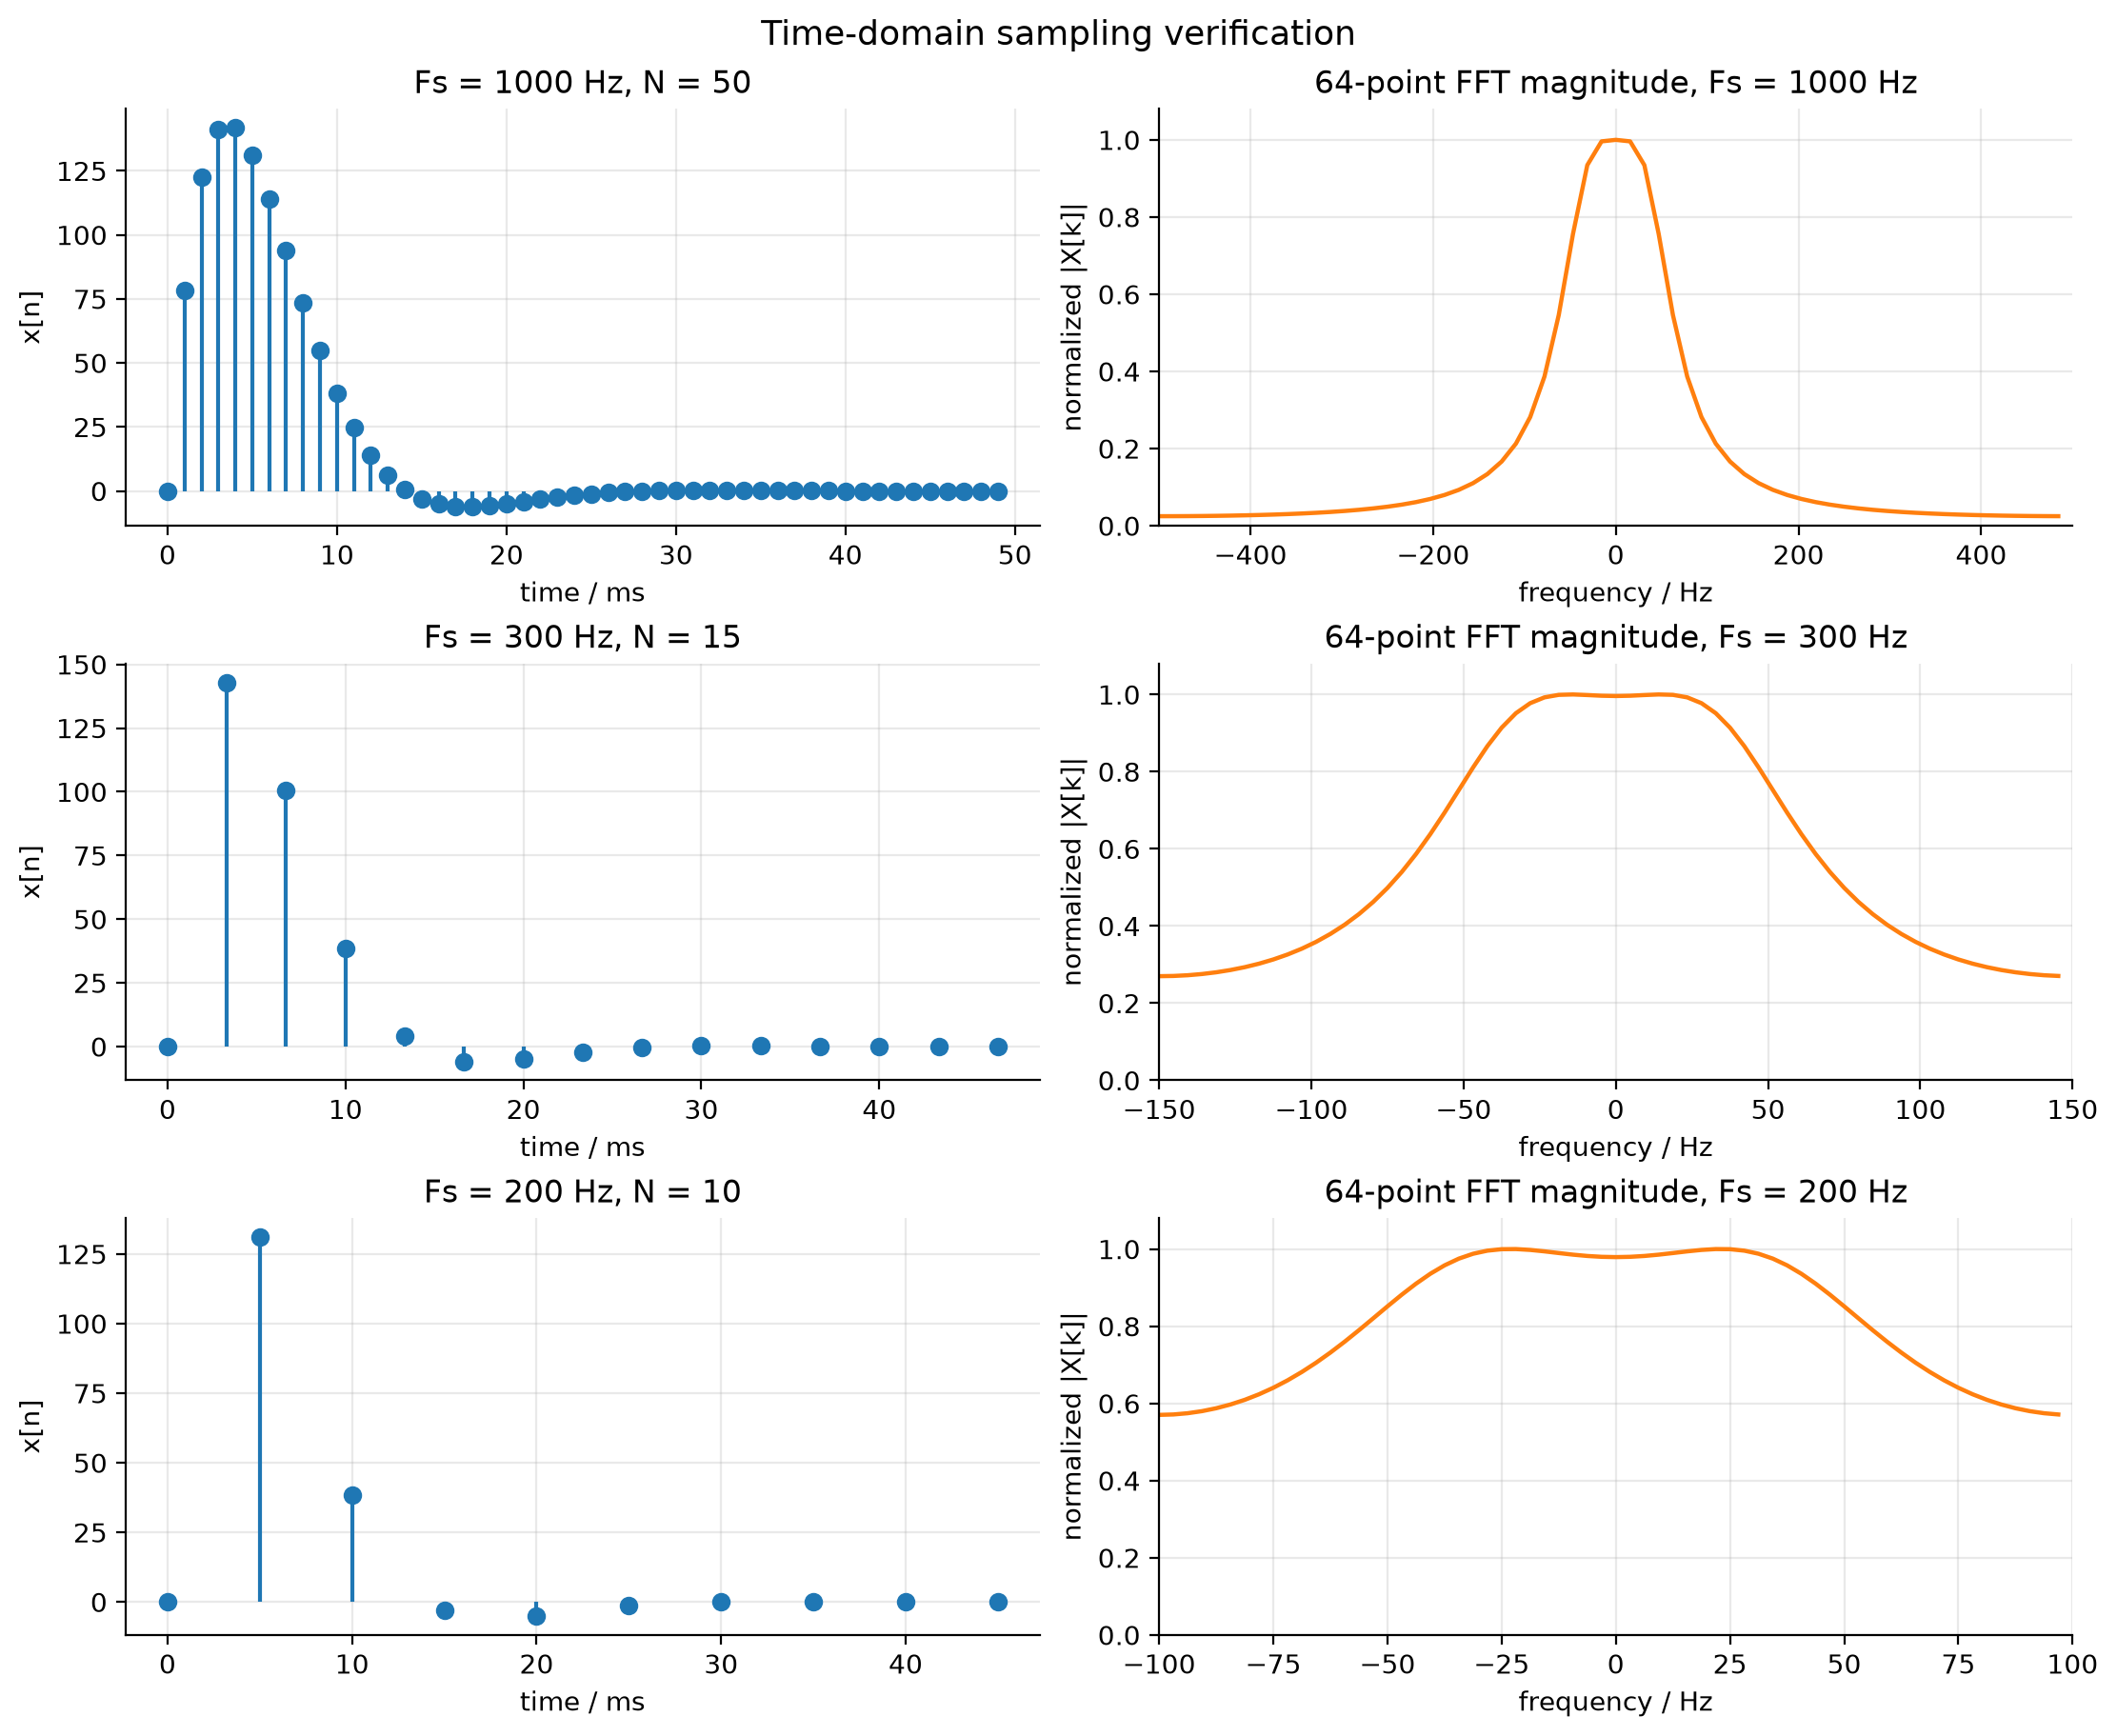
\includegraphics[width=0.95\textwidth]{time_domain_sampling.png}
\caption{不同采样频率下的采样序列和 64 点 FFT 幅频特性}
\label{fig:time-sampling}
\end{figure}

从图中可以看出，当 \(F_s=1000\,\Hz\) 时，采样点较密，奈奎斯特频率较高，采样后频谱在主频带内形状集中，未出现明显混叠。当 \(F_s=300\,\Hz\) 时，采样点数减少，频谱曲线明显变宽，频谱两侧的周期延拓成分开始对主频带产生影响，出现轻微混叠趋势。当 \(F_s=200\,\Hz\) 时，采样点数只有 10 点，奈奎斯特频率降低到 \(100\,\Hz\)，频谱周期延拓之间重叠明显，幅频特性发生较大变形，说明采样频率不足会造成频谱混叠。

由于该指数衰减正弦信号并不是严格带限信号，其频谱理论上有无限延伸的尾部，所以实际实验中应结合主要能量范围判断混叠程度。采样频率越高，周期延拓频谱之间的间隔越大，混叠越弱；采样频率越低，频谱重叠越明显，恢复原信号越困难。

\section{频域采样理论验证}

实验给定有限长序列
\begin{equation}
x(n)=
\begin{cases}
n+1, & 0\le n\le 13,\\
27-n, & 14\le n\le 26,\\
0, & \text{其他}.
\end{cases}
\end{equation}
该序列长度为 \(M=27\)。分别对 \(X(e^{j\omega})\) 在 \([0,2\pi]\) 上采样 32 点和 16 点，得到 \(X_{32}(k)\) 和 \(X_{16}(k)\)，再分别作 IFFT 得到 \(x_{32}(n)\) 和 \(x_{16}(n)\)。实验曲线如图 \ref{fig:freq-sampling} 所示。

\begin{figure}[H]
\centering
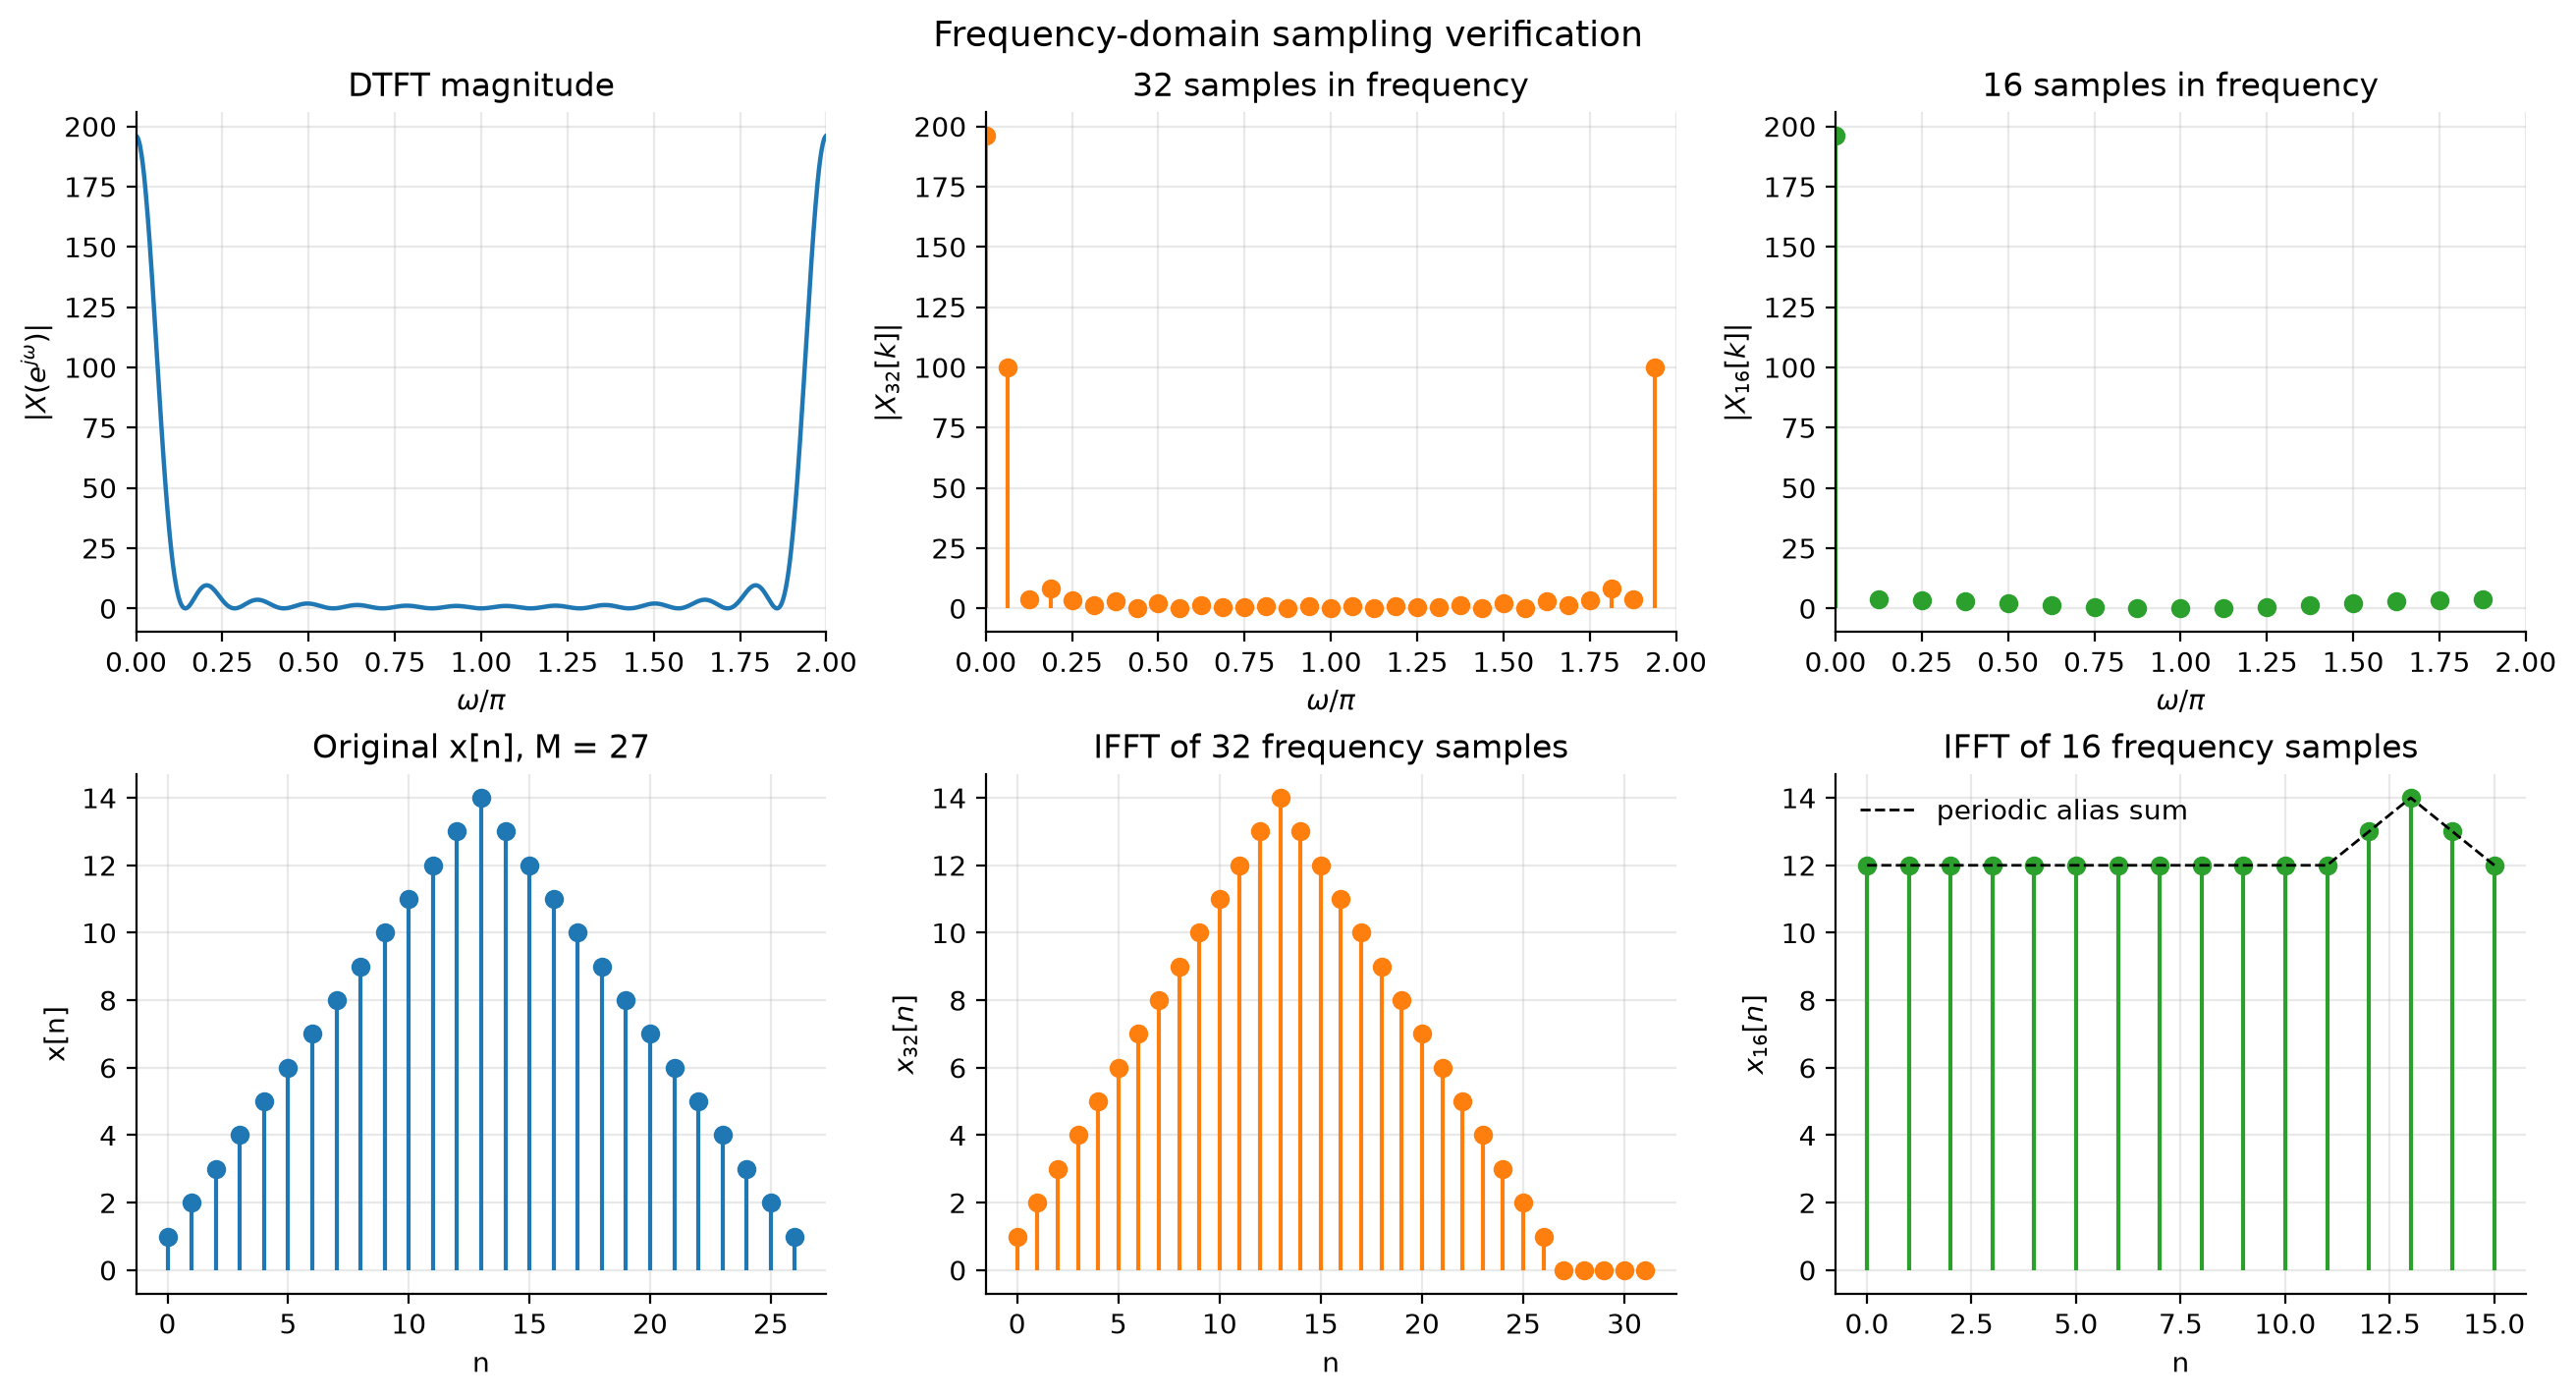
\includegraphics[width=0.96\textwidth]{frequency_domain_sampling.png}
\caption{频域采样及其 IFFT 结果}
\label{fig:freq-sampling}
\end{figure}

当 \(N=32\) 时，\(N>M\)，因此 32 点 IFFT 得到的 \(x_{32}(n)\) 与原序列 \(x(n)\) 相同，只是在尾部补了 \(32-27=5\) 个零点，没有发生时域混叠。

当 \(N=16\) 时，\(N<M\)，频域采样点数小于原序列长度。16 点 IFFT 得到的序列不是原序列的前 16 点，而是原序列按 16 为周期延拓后的主值区叠加结果：
\begin{equation}
x_{16}(n)=\sum_{r=-\infty}^{\infty}x(n+16r),\quad n=0,1,\cdots,15.
\end{equation}
计算得到
\[
x_{16}(n)=
[12,12,12,12,12,12,12,12,12,12,12,12,13,14,13,12].
\]
该结果与 16 点 IFFT 的输出一致，说明频域采样点数不足会在时域产生周期混叠。

\chapter{实验结论}

本实验分别验证了时域采样定理和频域采样定理。时域采样会使模拟信号频谱按采样频率周期延拓，采样频率越高，频谱副本之间间隔越大，越不容易发生混叠；采样频率过低时，频谱副本相互重叠，采样后信号无法完整表示原信号。使用 FFT 分析采样序列时，FFT 点数决定频域显示的离散频率刻度，补零可以使频谱曲线显示更平滑，但不能增加原采样数据中实际包含的信息。

频域采样会使时域序列周期延拓。若频域采样点数 \(N\ge M\)，IDFT 结果能保持原序列；若 \(N<M\)，IDFT 结果为原序列按 \(N\) 折叠后的叠加序列，会发生时域混叠。两个采样定理体现了傅里叶变换中的对偶关系：一个域中的离散采样，会导致另一个域中的周期延拓。

\chapter{思考题}

\section{当 \(N<M\) 时如何用一次最少点数的 DFT 得到频谱采样}

如果序列 \(x(n)\) 的长度为 \(M\)，希望得到其频谱 \(X(e^{j\omega})\) 在 \([0,2\pi]\) 上的 \(N\) 点等间隔采样，当 \(N<M\) 时，不能简单取原序列的前 \(N\) 点作 \(N\) 点 DFT，因为这样会丢掉后面的样值。

正确方法是先将原序列按模 \(N\) 折叠相加，得到长度为 \(N\) 的周期混叠序列：
\begin{equation}
x_N(n)=\sum_{r=-\infty}^{\infty}x(n+rN),\quad n=0,1,\cdots,N-1.
\end{equation}
然后对 \(x_N(n)\) 作一次 \(N\) 点 DFT：
\begin{equation}
X_N(k)=\sum_{n=0}^{N-1}x_N(n)e^{-j\frac{2\pi}{N}kn},
\quad k=0,1,\cdots,N-1.
\end{equation}
即可得到所需的频谱采样值
\begin{equation}
X_N(k)=X\left(e^{j\frac{2\pi k}{N}}\right).
\end{equation}
这里的一次 \(N\) 点 DFT 就是最少点数的 DFT，因为目标本身需要得到 \(N\) 个等间隔频域采样值。

\appendix
\chapter{程序清单}

\lstinputlisting[language=Python,caption={实验一 Python 程序},label={lst:program1}]{experiment1.py}

\end{document}
